\subsection{Evaluation}
To measure the quality of the classifications of the tool, the latest 8032 smart contracts\footnote{The date range of the contracts analyzed is from 20th of July 2018 to 6th of May 2018. Of those, 77 smart contracts were flagged as honeypots, which amounts to \( 0.96 \% \). The analysis time of a single smart contract amounted to less than a quarter of a second on a regular notebook.

\vspace{1em}
\begin{minipage}{\linewidth}
	\centering
	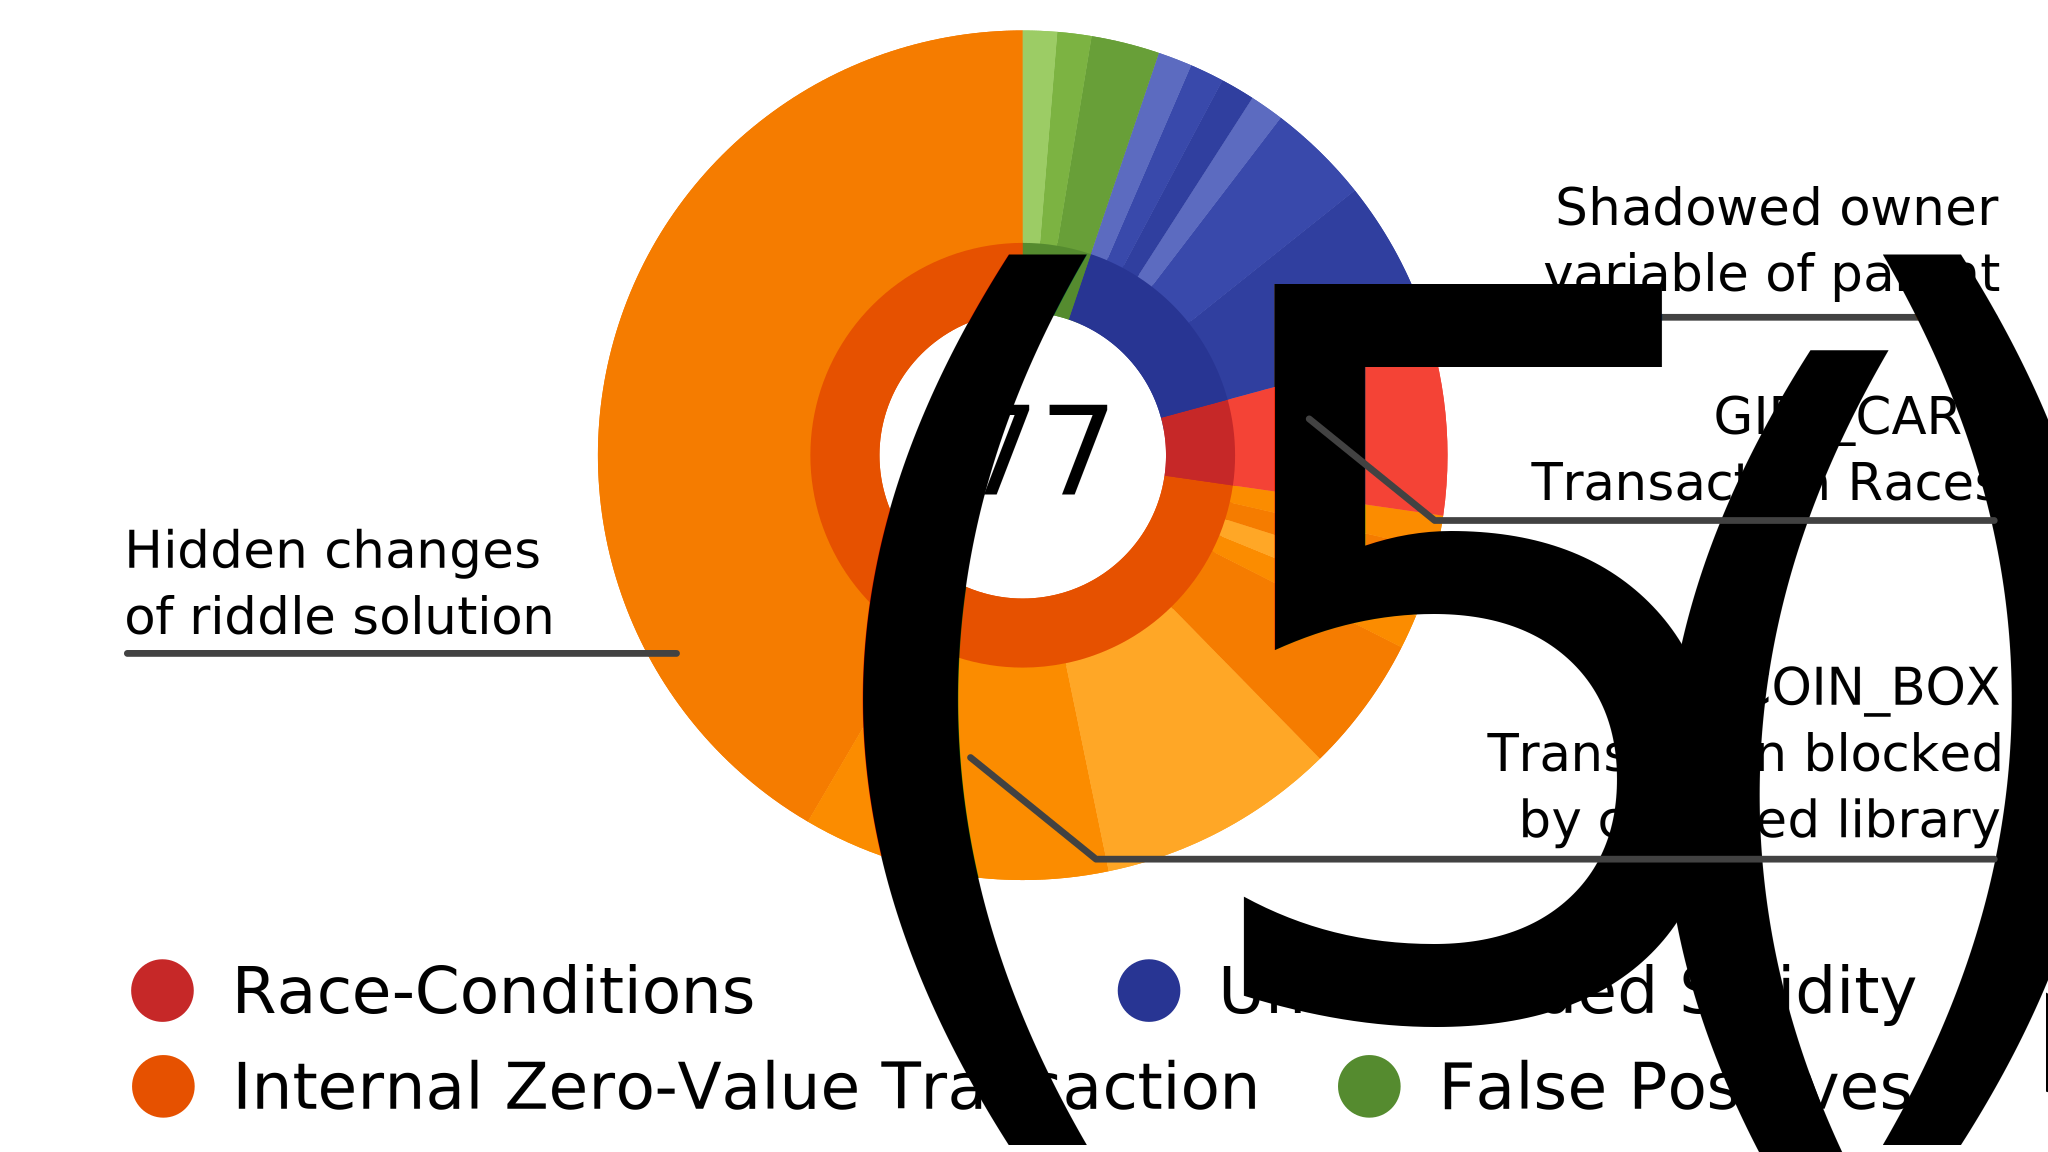
\includegraphics[width=9cm]{img/amphicyon/analysis.pdf}
	\captionof{figure}[Payload Layout]{Chart of manual analysis of the honeypot contracts. Different variants are printed in different shades in the outer circle.}
	\label{fig:honeypotchart}
\end{minipage}

All of the contracts found were manually analyzed and categorized; the results can be seen in \ref{fig:honeypotchart}. Four of the flagged smart contracts were harmless, which amounts to a false positive rate of \( 5.2 \% \). In the following, the findings of the manual analysis of the honeypots found by \textsc{Amphicyon} are presented in detail:\footnote{The notes on the manual classification can be found inside the folder \texttt{misc} in the repository.}

\paragraph{Found Honeypots}
Of those 73 found honeypots, many contracts were similar except for minor modifications like changed variable names and contract names. When considering unique findings, 15 distinct honeypots were found. Of those, seven had been already known before writing the paper, seven  contract types had not been known to the author, but other honeypots using the same technique had already been found. The use of race-conditions in honeypots as utilized in a multiple contracts called \texttt{GIFT_CARD}, of whom five instances were recognized, had not been known before running the tool; those contracts were detected because of some heuristics like silently failing functions as presented in section \ref{section:honeypots:silentlyfailing}.

With 56 of the honeypots their majority  abused zero-value transactions. 32 of them were identical riddle contracts, with names like \texttt{guess_and_get_the_money} (located at transaction \cite{etherscan:riddle}) where it seemed like Ether was transferred for the solution for a riddle like \mintinline{solidity}{"What do you serve that you can’t eat?"}, whose solution (here: \mintinline{solidity}{"guestS"}) was sent in plain text to the contract and then stored as a hashed value. To submit the solution and receive the bounty the user would have to pay 1 Ether; which would get stuck in the smart contract because the solution hash had been changed directly using an internal zero-value transaction. Also contracts similar to the smart contract called \texttt{COIN_BOX} presented in section \ref{section:honeypot:library} could be found seven times.

Five other tagged contracts found were identical honeypots called \texttt{GIFT_CARD} using transaction races, as presented in section \ref{section:honeypots:transactionordering}. The remaining twelve honeypots used various underhanded Solidity techniques: One each for uncalled call expressions, the empty string compiler bug and null pointer writing; nine of them used shadowed state variables.

The creators of honeypots yielded a considerable amount of crypto currencies: Of the manually validated contracts, 14 have been successful, totaling to a yield of 11.3 Ether or about 5.100 \$ in only about 11 weeks.\footnote{at \( 456.74 US\$ / Ether \) according to \cite{coinmarketcap:overview}}

\paragraph{General Findings}
There are also some other interesting results found in the analysis: More than three quarters of all smart contracts (6111 out of 8032) were recognized to interact with or to implement token contracts following the ERC20 or ERC223 interface.

The pattern of silently failing functions (a \mintinline{solidity}{if}-condition wrapping all the contents of a function instead of reverting the transaction using for example \mintinline{solidity}{require()} in the case the condition is not fulfilled) was present in almost all (72 out of 73) detected honeypots; but also in \( 7.5 \% \) (595 out of 7958) harmless contracts. In many cases this is unwanted behavior, for example forgetting to store  incoming payment or making the interacting user believe their function call was successful.

\paragraph{False Positives}
Four harmless contracts were marked as honeypots, three of those distinct. All of them contained common honeypot properties like the ability to transfer Ether and an easily understandable length. Additionally, all used silently failing functions, that could have been replaced by more user-friendly reverting checks, which made them more suspicious to \textsc{Amphicyon}, like\footnote{taken from \cite{etherscan:earlytokensale}}
\begin{minted}{solidity}
modifier afterDeadline() { if (now > deadline) _; }
\end{minted}

\paragraph{False Negatives}
To estimate the amount of false negatives, 20 honeypots that had been found during the research in discussion forums, blog posts or by chance have been checked. 19 of those contracts were recognized as honeypots, only one was a false negative: The similar variable names \mintinline{solidity}{payoutCursor_Id} and \mintinline{solidity}{payoutCursor_Id_} were detected in \texttt{FirePonzi} from section \ref{section:honeypots:similar}, but since using similar variable names were used too often in harmless contracts (the analysis counted 124 out of 7958 harmless contracts, and in nine out of 73 affected honeypots), this was not notable enough to be detected.
